\documentclass[twocolumns]{IEEEtran}
\usepackage{tikz}
\tikzstyle{box}=[rectangle,draw=black, ultra thick, minimum size=1cm]
\usepackage{algorithm}
\usepackage{algpseudocode}
\usepackage{graphicx}
\usepackage{caption}


\author{Alp Gokcek, Erdal Sidal Dogan, Mert Komurcuoglu\\gokcekal@mef.edu.tr, doganer@mef.edu.tr, komurcuoglum@mef.edu.tr\\ MEF University \\ \today}
\title{Rock-Paper-Scissors AI Agent}


\begin{document}
	\maketitle
	\begin{abstract}
		Maximum Subarray Sum is a well-known problem in the field of computer science. There are multiple number of solution algorithms with different complexities. In this paper, we demonstrated and compared 3 of these algorithms with quadratic, linear, and logarithmic complexities.
	\end{abstract}
\section{The Problem}
The Maximum Subarray Sum problem is the task of finding the contiguous subarray with largest sum in a given array of integers. Each number in the array could be positive, negative, or zero. For example: Given the array $[-2, 1, -3, 4, -1, 2, 1, -5, 4]$ the solution would be $[4, -1, 2, 1]$ with a sum of 6.
\section{Solutions}
\subsection{Brute-Force Approach}
This is the most intuitive solution to anyone. You basically traverse over the array and compare every possible combination of start and end index for the soultion array.\\ \\


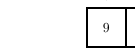
\begin{tikzpicture}[transform canvas={scale=.5}, trim left=-1cm]
[%%%%%%%%%%%%%%%%%%%%%%%%%%%%%%
box/.style={rectangle,draw=black, ultra thick, minimum size=0.5cm},
]%%%%%%%%%%%%%%%%%%%%%%%%%%%%%%

\foreach \x/\y in {0/9, 1/5,2/13,3/19,4/12,5/8,6/7,7/4,8/21,9/2,10/6,11/11}
\node[box] at (\x,0){\y};

\draw[->,very thick] (0,1.2) --  node[above,yshift=2mm]{start} (0,.7);
\draw[->,very thick] (1,1.2) --  node[above,yshift=2mm]{end} (1,.7);
\end{tikzpicture} 
\\ \\ \\
The \textit{start} index will be incremented by 1 everytime the \textit{end} index reaches the end of the array. Then the \textit{end} index will start from the element right next to the start element. At every iteration the sum between \textit{start} and \textit{end} indexes will be calculated. Hence, the maximum sum will be determined by computing every sum for the every possible sub-array. The complexity of this algorithm is $\mathcal{O}(n^3)$. With a little improvement we can convert this algorithm to be $\mathcal{O}(n^2)$. Instead of calculating the sum between two array indicies at every iteration from scratch, we know that the current sum will be the (current element + previous sum). Consequently, eliminating the loop which is used for calculating the sum from the algorithm will reduce the time complexity.
\newpage
\begin{algorithm}
	\caption{Brute-Force}
	\begin{algorithmic}[1]
		\State $n \leftarrow len(array)  $ \Comment{1}
		\State $max\_sum \leftarrow 0$ \Comment{1}
		\For {$i \leftarrow 1$ to $ n $} \Comment{$n+1$}
			\State $sum \leftarrow 0$ \Comment{$n$} 
			\For{$j \leftarrow i$ to $n$} \Comment{$\sum_{i = 0}^{n} (n - i + 2)$}
			\State $sum += array[j]$ \Comment{$\sum_{i = 0}^{n} (n - i + 1)$}
			\If{$sum > max\_sum$} \Comment{$\sum_{i = 0}^{n} (n - i + 1)$}
				\State $max\_sum \leftarrow sum$  \Comment{$\sum_{i = 0}^{n} (n - i + 1)$}
			\EndIf
			\EndFor
		\EndFor
	\end{algorithmic}
\end{algorithm}
\subsection{Divide \& Conquer Approach}
Another solution is to divide the array into half recursively and computing the max subarray sum for each half and the sub array for crossing both halfs. After calculating the summation for these 3 cases, we choose the largest one, thus we determine the maximum sub array.\\ 

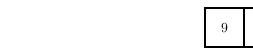
\begin{tikzpicture}[transform canvas={scale=.5}, trim left=-2.5cm]
	[%%%%%%%%%%%%%%%%%%%%%%%%%%%%%%
	box/.style={rectangle,draw=black, ultra thick, minimum size=0.5cm},
	]%%%%%%%%%%%%%%%%%%%%%%%%%%%%%%
	
	\foreach \x/\y in {0/9, 1/5,2/13,3/19,4/12,5/8,6/7,7/4}
	\node[box] at (\x,0){\y};
	
	%\draw[->,very thick] (0,1.2) --  node[above,yshift=2mm]{start} (0,.7);
	%\draw[->,very thick] (1,1.2) --  node[above,yshift=2mm]{end} (1,.7);
	\draw[->,very thick] (3.45,-.7) -- (1,-2);
	\draw[->,very thick] (3.55,-.7) -- (6,-2);
	
	\foreach \x/\y in {-1/9, 0/5,1/13,2/19}
	\node[box] at (\x,-3){\y};
	
	\foreach \x/\y in {5/12, 6/8,7/7,8/4}
	\node[box] at (\x,-3){\y};
	
	\draw[->,very thick] (0.45,-3.6) -- (-0.7,-4);
	\draw[->,very thick] (0.55,-3.6) -- (1.7,-4);
	
	\draw[->,very thick] (6.45,-3.6) -- (5.35,-4);
	\draw[->,very thick] (6.55,-3.6) -- (7.65,-4);
	
	\foreach \x/\y in {8/7,9/4}
	\node[box] at (\x,-5){\y};
	\foreach \x/\y in {4.5/12, 5.5/8}
	\node[box] at (\x,-5){\y};
	
	\foreach \x/\y in {-2/9,-1/5}
	\node[box] at (\x,-5){\y};
	\foreach \x/\y in {1.5/13,2.5/19}
	\node[box] at (\x,-5){\y};
	
	\draw[->,very thick] (8.45,-5.7) -- (7.95,-6.5);
	\draw[->,very thick] (8.55,-5.7) -- (9.05,-6.5);
	
	\draw[->,very thick] (4.95,-5.7) -- (4.45,-6.5);
	\draw[->,very thick] (5.05,-5.7) -- (5.55,-6.5);
	
	\draw[->,very thick] (2,-5.7) -- (2.5,-6.5);
	\draw[->,very thick] (2,-5.7) -- (1.5,-6.5);
	
	\draw[->,very thick] (-1.5,-5.7) -- (-1,-6.5);
	\draw[->,very thick] (-1.5,-5.7) -- (-2,-6.5);
	
	\foreach \x/\y in {-2.4/9}
	\node[box] at (\x,-7.2){\y};
	\foreach \x/\y in {-0.9/5}
	\node[box] at (\x,-7.2){\y};
	
	\foreach \x/\y in {1.2/13}
	\node[box] at (\x,-7.2){\y};
	\foreach \x/\y in {2.7/19}
	\node[box] at (\x,-7.2){\y};	
	
	\foreach \x/\y in {4.2/12}
	\node[box] at (\x,-7.2){\y};
	\foreach \x/\y in {5.7/8}
	\node[box] at (\x,-7.2){\y};	
	
	\foreach \x/\y in {7.8/7}
	\node[box] at (\x,-7.2){\y};
	\foreach \x/\y in {9.3/4}
	\node[box] at (\x,-7.2){\y};	
	
\end{tikzpicture} 
\\ \\ \\ \\ \\ \\ \\  \\ 

\begin{algorithm}
	\caption{Divide \& Conquer}
	\begin{algorithmic}[1]
		
	\Function {max\_crossing\_sub\_array} {$array, l, m, h$}
	\State$left\_max\_sum \leftarrow -100000$
	\State$sum\_l \leftarrow 0$
	\For{$ i \leftarrow m$ \textbf{downto} $l - 1$} 
		\State$sum\_l \leftarrow sum\_l + array[i]$
		\If{$sum\_l > left\_max\_sum$}
			\State $left\_max\_sum \leftarrow sum\_l$
		\EndIf
	\EndFor
	
	\State $sum\_r \leftarrow 0$
	\State $right\_max\_sum \leftarrow -100000$
	\For{$ j \leftarrow m + 1$ \textbf{to} $h + 1$} 
		\State$sum\_r \leftarrow sum\_r + array[j]$
		\If{$sum\_r > right\_max\_sum$}
			\State $right\_max\_sum \leftarrow sum\_r$
		\EndIf
	\EndFor\\
	\Return$left\_max\_sum + right\_max\_sum )$
	\EndFunction
	\\
	\Function{max\_sub\_array}{array, l, h}
		\State $m \leftarrow ((h + l) / 2)$
		\If{$l = h$} 
			\State \textbf{return} $array[l]$
		\EndIf
		
		\Return max(max\_subarray(array, l, m),\\
		max\_subarray(array, m + 1, h),\\
		max\_crossing\_subarray(array, l, m, h)\\
		)
	\EndFunction
	\end{algorithmic}
\end{algorithm}
\vspace{2cm}
The recurrence relation of the \textit{Divide \& Conquer algorithm} is as follows; 
$T(n) = 2T(n/2) + n $ \\ \\
By using \textit{Master's Method}, we conclude that this algorithm's complexity is $\mathcal{O}(n\log n)$
\newpage
\subsection{Linear Time}
Another solution is by just traversing the array once and comparing the current element with maximum sub array ending there. Since the problem is finding the maximum contiguous subarray, we pick the larger one, a.k.a Kadane’s Algorithm.
The complexity is calculated as the summation of the costs of all the lines;
$ C_1 + C_2 +C_3 + C_4 + n(C_4 + C_5 + C_6 + C_7 + C_8 + C_9) = \mathcal{O}(n) $
Where $C_n$ denotes the cost of the line $n$.
\begin{algorithm}
	\caption{Linear Time}
	\begin{algorithmic}[1]
	\State$max\_so\_far \leftarrow -100000$ \Comment{$1$}
	\State$max\_ending\_here \leftarrow -100000$ \Comment{$1$}
	\State$n \leftarrow length(array)$ \Comment{$1$}
		\For {$i \leftarrow 1$ to $ n $}  \Comment{$n + 1$}
			\State$max\_ending\_here \leftarrow max\_ending\_here + array[i]$ \Comment{$n$}
			\If{$max\_ending\_here < array[i]$}\Comment{$n$} 
					\State$max\_ending\_here \leftarrow array[i]$\Comment{$n$}
			\EndIf
			\If{$max\_so\_far < max\_ending\_here$} \Comment{$n$}
				\State$max\_so\_far max\_ending\_here$ \Comment{$n$}
			\EndIf

		\EndFor
	\end{algorithmic}
\end{algorithm}


\section{Comparisons}
\begin{center}
	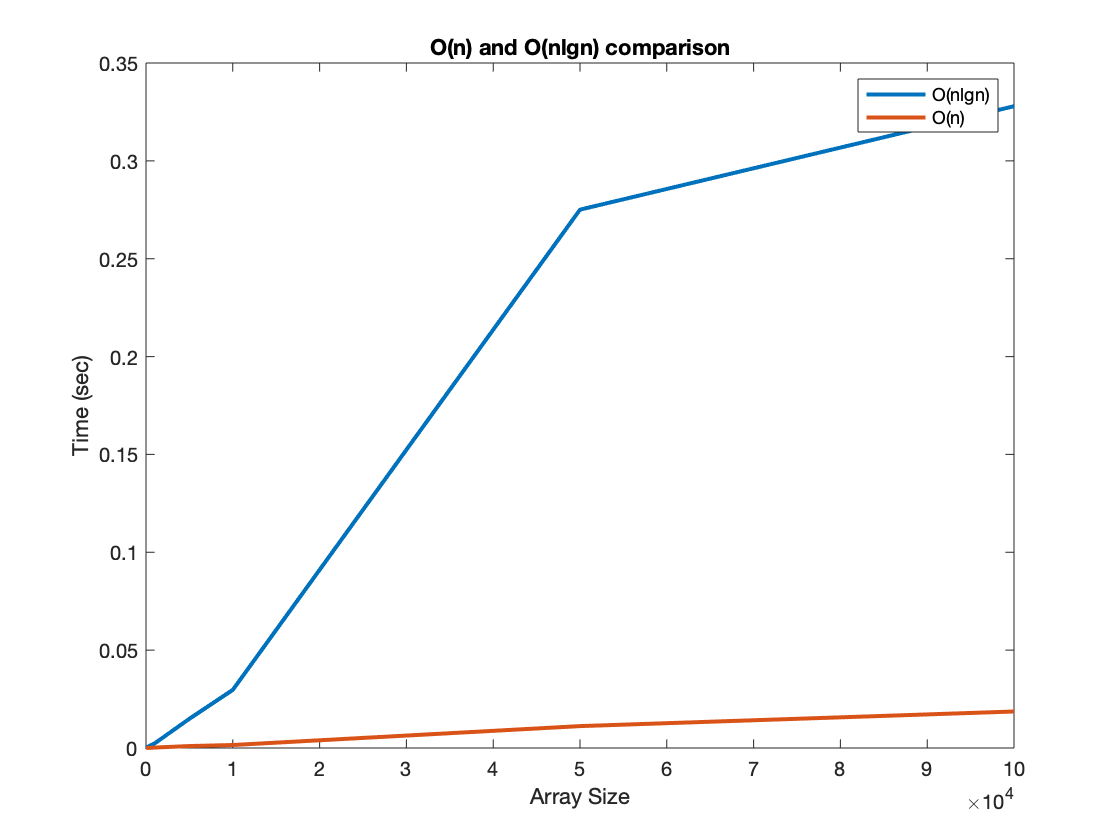
\includegraphics[scale=0.22]{n_nlgn.png}\label{n}
	\captionof{figure}{Divide \& Conquer Algorithm ($\mathcal{O}(n\log n)$) vs Linear Time Algorithm ($ \mathcal{O}(n)$)}
	
	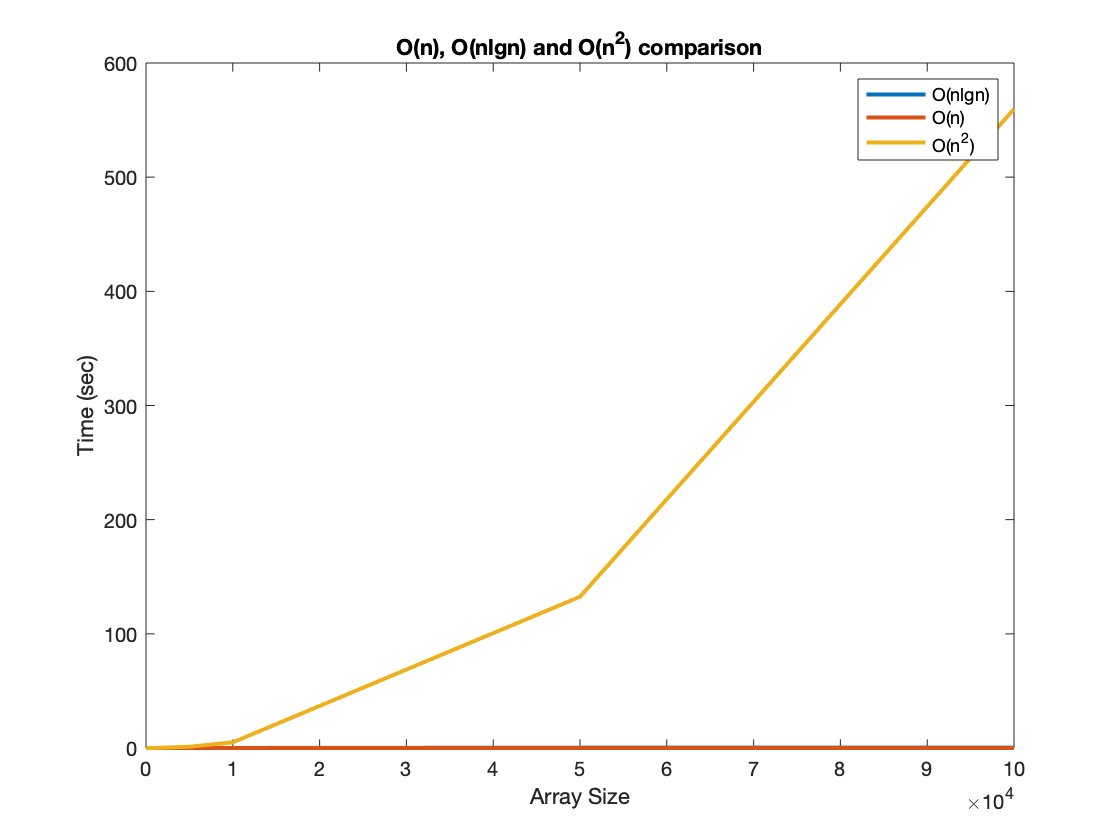
\includegraphics[scale=.22]{n_nlgn_n2.png}\label{n2}
	\captionof{figure}{Brute-Force ($\mathcal{O}(n^2)$)vs. Divide \& Conquer ($\mathcal{O}(n\log n)$) vs Linear Time ($ \mathcal{O}(n)$)}
\end{center}
As the Fig. 1 and Fig. 2 indicates, Brute-Force algorithm is way slower comparing to D\&C and Linear Time algorithms, espicially in larger data sets. 
\section{References}

[1]"Maximum Subarray Sum using Divide and Conquer algorithm - GeeksforGeeks", GeeksforGeeks, 2019. [Online]. Available: https://www.geeksforgeeks.org/maximum-subarray-sum-using-divide-and-conquer-algorithm/. [Accessed: 17- Nov- 2019].\\

[2]M. Talluri, "Kadane’s Algorithm Explained", Hackernoon.com, 2019. [Online]. Available: https://hackernoon.com/kadanes-algorithm-explained-50316f4fd8a6. [Accessed: 17- Nov- 2019].\\

[3]R.Singhal, "Kadane’sAlgorithm (Dynamic Programming) How and Why does it Work?", Medium, 2018.[Online]. Available:https://medium.com/@rsinghal757/kadanes-algorithm-dynamic-programming-how-and-why-does-it-work-3fd8849ed73d. [Accessed: 17- Nov- 2019].



\end{document}